% !TEX program = pdflatex
\documentclass[conference]{IEEEtran}

% Packages
\usepackage[utf8]{inputenc}
\usepackage[T1]{fontenc}
\usepackage{amsmath,amssymb}
\usepackage{graphicx}
\usepackage{booktabs}
\usepackage{xcolor}
\usepackage{hyperref}
\usepackage{float}
\usepackage{tikz}
\usetikzlibrary{arrows.meta,positioning,shapes.geometric}
\graphicspath{
{figures/search/}
{figures/rq1/}
{figures/ablations/}
{figures/routing/}
{figures/flops/}
{figures/training/}
{figures/}
{paper/figures/}
{../development/experiments/plots/search/}
{../development/experiments/plots/rq1/}
{../development/experiments/plots/ablations/}
{../development/experiments/plots/routing/}
{../development/experiments/plots/flops/}
{../development/experiments/plots/training/}
{../development/experiments/plots/}
{development/experiments/plots/search/}
{development/experiments/plots/rq1/}
{development/experiments/plots/ablations/}
{development/experiments/plots/routing/}
{development/experiments/plots/flops/}
{development/experiments/plots/training/}
{development/experiments/plots/}
}

\hypersetup{colorlinks=true, linkcolor=blue, citecolor=blue, urlcolor=blue, hypertexnames=false}

% ============================================================================
\begin{document}

\title{Neural Architecture Search for Joint Big/Little\\Dynamic Inference Networks}

\author{
    \IEEEauthorblockN{Kristoffer Petersen, Oliver Larsen, Oliver Svendsen, Aleksander Korsholm}
    \IEEEauthorblockA{
        University of Southern Denmark (SDU)\\
        \textit{Supervisors:} Emil Jørgensen Njor, Francesco Daghero
    }
}

\maketitle
\thispagestyle{plain}
\pagestyle{plain}

% ============================================================================
\begin{abstract}
Edge and battery-powered systems increasingly run deep neural networks
on-device, where strict memory, latency, and energy budgets constrain how
much computation each input is allowed
reduces the average cost by adapting computation to input difficulty: a
small ``little'' network handles easy inputs, and harder inputs are
deferred to a larger ``big'' network. Designing such a big/little
cascade is a coupled problem. The two networks must share a routing rule,
a memory budget, and a calibration behaviour, yet most existing work
either places multiple exits inside a single backbone or composes a
cascade from networks trained independently. We ask whether the little
and big networks should instead be searched \emph{jointly} as a cascade
pair under explicit microcontroller (MCU) deployment constraints. We
propose a constrained NSGA-II co-search that selects
little/big CNN pairs on CIFAR-10 and compare it against an independent
NAS baseline. At a fixed routing threshold $\tau=0.70$, the joint cascade
reaches 80.69\% accuracy at 2.08~M MACs against 74.03\% at 2.22~M MACs
for the independent baseline. Deployed on a 512~KiB microcontroller, the
joint cascade further reduces measured runtime by 23\% and route-aware
energy by 22\% over the same baseline.
\end{abstract}

% ============================================================================
\section{Introduction}
\label{sec:introduction}

Deep neural networks have grown both more accurate and more expensive
\cite{he2016resnet,tan2019efficientnet}. The same models that deliver strong
predictions in the cloud are increasingly being asked to run on-device, on
microcontrollers and other battery-powered embedded systems where a typical
flash and SRAM budget is under one megabyte and average inference energy is a
first-class constraint \cite{warden2019tinyml,david2021tflm,lin2020mcunet}.
Always-on classification, keyword spotting, and sensor processing in this
``TinyML'' regime has motivated benchmarks and tooling for on-device deep
learning \cite{banbury2021mlperftiny}, but the gap between
state-of-the-art network capacity and microcontroller resources remains large.

\emph{Dynamic inference} narrows this gap by spending compute only where it
is needed. Rather than running a fixed network on every input, a dynamic
network adapts the inference path to each sample
\cite{han2021dynamic,bolukbasi2017adaptive}. A big/little cascade is one of
the simplest such designs \cite{park2015biglittle}: a cheap ``little''
network is evaluated on every input, and a more expressive ``big'' network
is invoked only when the little network is uncertain. The cascade can decide
this route with a learned gate \cite{regol2024jeidnn,wang2018skipnet}, a
margin-based rule \cite{bolukbasi2017adaptive}, or a confidence threshold
\cite{teerapittayanon2017branchynet,kaya2019shallowdeep}.We use a
maximum-softmax confidence threshold because it requires no extra routing
model, has negligible runtime overhead, and is straightforward to deploy
under embedded constraints. The full routing rule is given in
Section~\ref{sec:background:routing}. Such a cascade reduces average compute
only if the little network is accurate on easy samples, the big network is
strong on deferred samples, and the threshold routes examples correctly.

Designing such cascades is not just a matter of finding two accurate
models. The two models must work together under a shared routing rule and a
shared deployment budget. If the little model is too small, it may rarely exit
correctly. If the big model receives too much capacity, the cascade may become
accurate but expensive. If the confidence threshold is too low, confident
wrong exits can damage accuracy; if it is too high, most samples defer and the
cascade loses its computational benefit. These trade-offs make cascade design a
multi-objective problem involving accuracy, MACs, exit ratio, memory, and
calibration.

Neural architecture search (NAS) is a natural tool for this setting because it
can explore many architectural design choices under explicit constraints
\cite{elsken2019nassurvey}. Prior work has studied NAS for efficient models,
multi-objective architecture search, and dynamic inference, including early-exit
networks and model cascades \cite{deb2002nsga2,lu2019nsganet,chebykin2022encas}.
However, many cascade systems either design models independently or focus on
placing exits inside a single backbone (Table~\ref{tab:related-comparison}).
This leaves open the question of whether
a little and big model should be searched jointly as a pair, so that the search
objective directly reflects cascade behavior.

This report studies that question on CIFAR-10 under an edge-style deployment
constraint. We compare a joint co-search method, in which NSGA-II searches
complete little/big pairs against cascade accuracy and expected cascade MACs
directly, against an independent baseline that searches the two roles
separately as standalone classifiers and combines them afterwards. Both
methods share the underlying CNN search space, the same
\emph{proxy-training} budget (a short 5-epoch run used only to rank
candidates during search; final claims use full retraining), and the
deployment constraints. The comparison therefore isolates the effect of
\emph{searching as a cascade} from the effect of architectural capacity.

Architecture search is only part of the problem, however, because cascade
routing depends on confidence. Cross-entropy (CE) optimizes classification
accuracy but does not reflect the fact that some samples should exit at the
little model while others should defer, and miscalibrated confidence
translates directly into harmful early exits
\cite{guo2017calibration,mueller2019labelsmoothing,li2021learningtocascade}.
We therefore retrain the selected joint architectures under four objectives:
CE, CE with label smoothing, a cascade-aware co-training loss, and the
cascade-aware loss combined with label smoothing. These choices are not
fully orthogonal: the cascade-aware loss is itself confidence-shaping and
interacts with the architecture's routing behaviour at the same threshold, so RQ2 is studied as an ablation over a fixed set of selected
architectures rather than as an independent optimisation.

The report is organised around two research questions:

\begin{itemize}
    \item \textbf{RQ1:} Does joint NAS co-search of a little/big model pair
    produce a better final cascade accuracy versus average cascade MACs
    trade-off than independently searched and combined model pairs under
    matched search spaces and edge-memory constraints?

    \item \textbf{RQ2:} After architectures are selected by joint NAS, does
    cascade-aware co-training improve cascade accuracy, routing quality, or
    calibration compared with standard CE and CE with label smoothing?
\end{itemize}

We also analyse how the operating threshold $\tau$, the resulting exit
ratio, and the little-model calibration jointly shape the deployed
accuracy MACs trade-off. This is a follow-up analysis on the selected
joint cascades rather than a separate research question.

The implementation and experiment scripts are available in the project
repository.\footnote{\href{https://github.com/Neural-Efficiency-Research-Unit-NERU/nas-dynamic-big-little-cascade}{Neural-Efficiency-Research-Unit-NERU/nas-dynamic-big-little-cascade}}

\medskip\noindent\textbf{Contributions.} This work makes the following
contributions:
\begin{enumerate}
    \item A joint NSGA-II co-search procedure for big/little CNN cascades
    under a 450~KiB combined weight-plus-activation budget motivated by a
    512~KiB MCU. The comparison keeps the search space, proxy budget, and
    deployment constraints matched between joint and independent NAS.

    \item A cascade-aware co-training loss that replaces the hard routing
    decision with a soft exit probability based on the little network's
    confidence, so that little-model and big-model cross-entropy are
    weighted by the route a sample is likely to take. Treated as an
    ablation (conditions C1-C4 in
    Section~\ref{sec:methodology:loss-ablations}), it shows how retraining
    choices shift the same selected architectures between cheaper and more
    accurate operating points.

    \item A microcontroller deployment study on a Raspberry Pi Pico 2
    connecting the analytical accuracy-MACs frontier to measured runtime
    and route-aware energy while fitting within the TensorFlow Lite Micro
    \cite{david2021tflm} memory arenas of the target.

    \item An analysis of how threshold $\tau$, exit ratio $\rho$, calibration
    (ECE, Section~\ref{sec:background:ece}), and routing error jointly shape
    the deployed accuracy-MACs trade-off, explaining why a high exit ratio
    on the independent baseline does not translate into a stronger cascade.
\end{enumerate}

The remainder of the report is structured as follows.
Section~\ref{sec:background} introduces the background concepts shared by the
rest of the paper (threshold-routed cascades, neural architecture search, and
calibration). Section~\ref{sec:related} reviews dynamic inference, NAS for
efficient models, and confidence calibration for cascade routing.
Section~\ref{sec:methodology} describes the search space, the joint and
independent NAS procedures, and the cascade-aware loss.
Section~\ref{sec:experiments} presents the experimental setup and evaluation
metrics. Section~\ref{sec:results} reports the results for the two research
questions and the supporting routing analysis. Section~\ref{sec:discussion} discusses the main findings,
limitations, and future work, and Section~\ref{sec:conclusion} concludes the
report.

% ============================================================================
\section{Background}
\label{sec:background}

This section defines the components shared by the rest of the paper: the
big/little cascade routing rule, the architecture-search formulation, and the
calibration metric used to interpret confidence-based routing.

\subsection{Big/Little Cascade Routing}
\label{sec:background:routing}

A big/little cascade chains a lightweight \emph{little} model with a larger
\emph{big} model that acts as a fallback for samples the little model is
uncertain about \cite{park2015biglittle}. For each input $x$, the little model
is evaluated first and produces logits $z_l$. We use the \emph{max-softmax}
confidence,
\begin{equation}
c_l = \max(\mathrm{softmax}(z_l)),
\label{eq:max-softmax}
\end{equation}
because it requires no auxiliary gating network, adds negligible runtime
overhead, and is straightforward to evaluate on embedded targets
\cite{guo2017calibration,teerapittayanon2017branchynet}. The cascade applies
a fixed threshold $\tau$: if $c_l > \tau$, the little model's prediction
$\hat{y}_l$ is accepted and the cascade exits. Otherwise the input is
deferred to the big model, which produces logits $z_b$ and prediction $\hat{y}_b$. This
threshold rule is illustrated in Figure~\ref{fig:cascade-routing}.

\begin{figure}[t]
\centering
\resizebox{\columnwidth}{!}{%
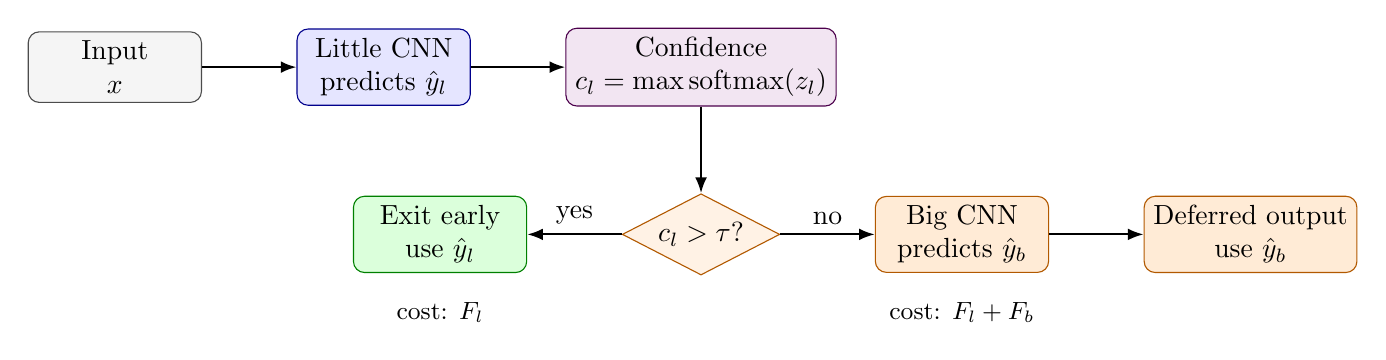
\begin{tikzpicture}[
    node distance=1.1cm and 1.2cm,
    box/.style={
        draw,
        rounded corners,
        align=center,
        minimum width=2.2cm,
        minimum height=0.8cm
    },
    inputbox/.style={box, fill=gray!8, draw=gray!60!black},
    littlebox/.style={box, fill=blue!10, draw=blue!55!black},
    confbox/.style={box, fill=violet!10, draw=violet!60!black},
    exitbox/.style={box, fill=green!14, draw=green!50!black},
    bigbox/.style={box, fill=orange!16, draw=orange!70!black},
    decision/.style={
        draw,
        diamond,
        aspect=1.8,
        align=center,
        inner sep=1.2pt,
        minimum width=2.0cm,
        fill=orange!10,
        draw=orange!70!black
    },
    arrow/.style={-{Latex[length=2mm]}, thick}
]
\node[inputbox] (input) {Input\\$x$};
\node[littlebox, right=of input] (little) {Little CNN\\predicts $\hat{y}_l$};
\node[confbox, right=of little] (conf) {Confidence\\$c_l=\max \mathrm{softmax}(z_l)$};
\node[decision, below=of conf] (gate) {$c_l > \tau$?};
\node[exitbox, left=of gate] (exit) {Exit early\\use $\hat{y}_l$};
\node[bigbox, right=of gate] (big) {Big CNN\\predicts $\hat{y}_b$};
\node[bigbox, right=of big] (final) {Deferred output\\use $\hat{y}_b$};

\draw[arrow] (input) -- (little);
\draw[arrow] (little) -- (conf);
\draw[arrow] (conf) -- (gate);
\draw[arrow] (gate) -- node[above] {yes} (exit);
\draw[arrow] (gate) -- node[above] {no} (big);
\draw[arrow] (big) -- (final);

\node[align=center, below=0.25cm of exit] {\small cost: $F_l$};
\node[align=center, below=0.25cm of big] {\small cost: $F_l+F_b$};
\end{tikzpicture}%
}
\caption{Threshold-based routing in the big/little cascade. Every sample pays
the little-model cost $F_l$; green denotes the early-exit path for samples
with $c_l > \tau$, while orange denotes the deferred path that additionally
pays the big-model cost $F_b$.}
\label{fig:cascade-routing}
\end{figure}

Let $\rho \in [0,1]$ denote the \emph{exit ratio}, the fraction of samples
handled by the little model alone. The expected per-sample compute cost
(measured in multiply-accumulate operations, MACs) is then
\begin{equation}
F_{\mathrm{cascade}} = F_l + (1-\rho)\, F_b,
\label{eq:cascade-cost}
\end{equation}
where $F_l$ and $F_b$ are the analytical MAC counts of the little and big
models. The first term is paid on every input; only the deferred fraction
$1-\rho$ pays the big-model cost \cite{park2015biglittle,han2021dynamic}.

\subsection{Neural Architecture Search}
\label{sec:background:nas}

Neural Architecture Search (NAS) refers to a class of \emph{algorithms} that
automate architecture design \cite{elsken2019nassurvey}. A NAS algorithm is
defined by three components: a \emph{search space} of candidate architectures,
a \emph{search strategy} that explores it, and a \emph{performance-estimation
method} that scores candidates. Modern NAS methods range from
reinforcement-learning controllers \cite{zoph2017nasrl}, through evolutionary
algorithms \cite{real2019regevo,deb2002nsga2}, to differentiable relaxations
\cite{liu2019darts} and weight-sharing supernetworks \cite{pham2018enas}.
Because full retraining of every candidate is computationally prohibitive,
practical NAS uses a proxy: a short training run (here, 5 epochs) whose final
accuracy is used as a ranking signal for the search, with longer retraining
applied only to the selected architectures
\cite{real2019regevo,liu2019darts}. NAS additionally optimizes
non-accuracy targets such as MACs, memory, or latency
\cite{lu2019nsganet,chebykin2022encas,benmeziane2021hwnas}; In this report, we use NSGA-II, a multi-objective algorithm\cite{deb2002nsga2}, because it can evaluate architectures using more than one objective at the same time, such as accuracy and compute cost. This makes it suitable for mixed discrete architecture variables and produces an explicit Pareto front for the accuracy-compute trade-off.


\subsection{Confidence Calibration and Expected Calibration Error}
\label{sec:background:ece}

A classifier is \emph{well calibrated} when its predicted confidence matches
its empirical accuracy: among samples with $c_l \approx 0.7$, the model should
be correct about 70\% of the time. Modern deep networks are typically
overconfident \cite{guo2017calibration}, which is consequential for cascades
because miscalibrated confidence directly biases the threshold router toward
unsafe early exits \cite{li2021learningtocascade}. We quantify calibration
using Expected Calibration Error (ECE) \cite{naeini2015ece,guo2017calibration}.
Test samples are sorted by predicted confidence and grouped into $K$
equal-width bins $B_1,\dots,B_K$; ECE is the
weighted gap between the average confidence and the average accuracy in each
bin,
\begin{equation}
\mathrm{ECE} = \sum_{k=1}^{K} \frac{|B_k|}{N}\,
\bigl|\mathrm{acc}(B_k) - \mathrm{conf}(B_k)\bigr|.
\label{eq:ece}
\end{equation}
We use $K=15$ bins, following common practice \cite{guo2017calibration}, and
report ECE for the little model since its confidence is the quantity the
threshold router actually consumes.

% ============================================================================
\section{Related Work}
\label{sec:related}

\subsection{Dynamic Inference and Big/Little Cascading}
\label{sec:related:dynamic}

Dynamic neural networks adapt their computation to each input instead of using a
fixed inference path for all samples. Han et al.\ survey this area and group
dynamic models into instance-wise, spatial-wise, and temporal-wise adaptation
methods \cite{han2021dynamic}. Big/little cascades are an instance-wise dynamic
inference method: an inexpensive model handles easy samples, while difficult
samples are routed to a more expensive model. Park et al.\ proposed an early
big/little DNN system for low-power inference, showing that a small network can
filter easy inputs before invoking a larger network \cite{park2015biglittle}.
This idea is attractive for embedded systems because the expected cost depends
on the exit ratio, not only on the worst-case cost of the largest model.

Closely related work studies early-exit networks, where auxiliary classifiers
are attached to intermediate layers of a single backbone. BranchyNet introduced
side branches that allow confident samples to exit before reaching the final
layer \cite{teerapittayanon2017branchynet}. MSDNet extends this idea with
multi-scale feature representations for anytime and budgeted classification
\cite{huang2018msdnet}. Shallow-Deep Networks analyze ``overthinking'', where a
deep network can change an already-correct intermediate prediction into an
incorrect final one, and use early exits to reduce unnecessary computation
\cite{kaya2019shallowdeep}. These methods demonstrate the value of adaptive
computation, but they primarily modify a single backbone. Our work instead
studies a cascade of two independent CNNs and asks how capacity should be
allocated between the little and big models.

The routing rule is central to both early-exit networks and model cascades.
Most systems use confidence thresholds: a sample exits if the intermediate or
little model is sufficiently confident. This makes calibration important,
because overconfident wrong predictions directly become wrong early exits.
Learning to Cascade addresses this issue by calibrating confidence specifically
for cascade systems, showing that standard calibration methods do not always
optimize the accuracy-cost trade-off of a cascade \cite{li2021learningtocascade}.
This motivates our separate analysis of confidence, routing errors, and
retraining losses.

% Related-work subsection divider
\subsection{NAS for Dynamic Inference}
\label{sec:related:nasdynamic}

NAS automates architecture design using a defined search space, a search
strategy, and a performance-estimation method \cite{elsken2019nassurvey}. It is
particularly relevant for dynamic inference because accuracy and compute must be
optimized jointly. Multi-objective evolutionary NAS is a common fit for this
setting, since it can produce a Pareto front rather than a single scalarized
solution. NSGA-II is a standard elitist multi-objective genetic algorithm
\cite{deb2002nsga2}, and NSGA-Net applies multi-objective evolutionary search
to neural architectures \cite{lu2019nsganet}. We follow this general
multi-objective view, but apply it to cascade pairs under explicit memory and
parameter constraints.

Several recent methods apply NAS to early-exit neural networks. EDANAS searches
early-exit networks by adapting an Once-for-All style search space and jointly
considering accuracy and MACs \cite{gambella2023edanas}. NACHOS extends this
line toward hardware-constrained early-exit design, searching for networks that
satisfy accuracy and MAC constraints at inference time
\cite{gambella2025nachos}. These approaches are close in spirit because they
use architecture search for adaptive inference. However, they focus on adding
or optimizing exits within a single network. Our method searches two separate
role-specific networks and optimizes their behavior as a cascade pair.

Other work focuses on learning the exit decision itself. JEI-DNN jointly learns
the gating mechanism and intermediate inference modules, addressing the
train-test mismatch that arises when confidence-threshold gates are trained
separately from the prediction modules \cite{regol2024jeidnn}. This line of
work is complementary to ours: JEI-DNN improves learned gating inside dynamic
neural networks, while our study keeps a simple threshold router and asks
whether the architectures of the two cascade members should be searched jointly.

ENCAS is the closest related work on NAS for model cascades. It performs
evolutionary neural cascade search across pretrained supernetworks to obtain a
front of cascades trading accuracy against MACs \cite{chebykin2022encas}. Our
work differs in two ways. First, we co-search the little and big models from a
small role-specific CNN search space under a strict edge-memory budget, rather
than composing subnetworks from pretrained supernetworks. Second, we explicitly
compare joint co-search against an independently searched baseline and then
study whether cascade-aware retraining improves the selected architectures.

% Related-work subsection divider
\subsection{Confidence Calibration for Cascade Routing}
\label{sec:related:calibration}

Modern neural networks are often miscalibrated: their predicted probabilities
can be more confident than their empirical accuracy \cite{guo2017calibration}.
This is especially important for cascades because the confidence score is not
only a diagnostic quantity, since it controls computation. A poorly calibrated little
model can exit on samples that should have been deferred to the big model. As a
result, optimizing standalone classification accuracy is not necessarily enough
to optimize cascade accuracy.

Label smoothing is one common training modification that can affect both
accuracy and calibration. Muller et al.\ show that label smoothing changes the
structure of learned representations and can improve generalization, although
its effect depends on the task and downstream use \cite{mueller2019labelsmoothing}.
Focal loss has also been studied as a calibration-aware alternative; Mukhoti et
al.\ show that it can improve calibration in some settings
\cite{mukhoti2020calibrating}. These results motivate treating the final
training objective as part of the cascade design, rather than evaluating only
the searched architecture.

to model accuracy \cite{li2021learningtocascade}. This distinction matters
because confidence is also the routing signal: an overconfident little model
can save compute but produce an incorrect early exit, while an underconfident
little model may defer too often and lose the computational benefit of the
cascade. A useful confidence score should therefore separate samples the little
model can handle from samples that are worth sending to the big model. Our
cascade-aware loss follows the same motivation but is used as a retraining
objective for a jointly searched big/little pair. It introduces soft routing
weights during training so that little-model and big-model losses are weighted
according to the expected route of each sample. The goal is to improve cascade
behavior without replacing the simple threshold rule used at inference.


% Related-work subsection divider
\subsection{Resource-Constrained NAS}
\label{sec:related:hwnas}

Hardware-aware NAS extends architecture search with deployment constraints such
as latency, memory, energy, MACs, or parameter count. This is important because
the most accurate architecture under an unconstrained search is often not
deployable on edge hardware. Surveys of hardware-aware NAS describe how search
objectives can be coupled to device-specific measurements or analytical proxies
\cite{benmeziane2021hwnas}. NetAdapt iteratively adapts a pretrained network to
meet platform constraints \cite{yang2018netadapt}, while ProxylessNAS searches
directly on the target task and hardware instead of relying only on proxy tasks
\cite{cai2019proxylessnas}. MobileNetV3 combines platform-aware search with
efficient mobile building blocks \cite{howard2019mobilenetv3}.

During NAS, our search uses analytical resource constraints rather than measured
latency: deployment memory, parameter count, and average cascade MACs. This
keeps architecture selection reproducible and independent of measurement noise
from a specific hardware run. Measured Pico 2 latency is treated separately as a
deployment evaluation after model selection. The memory constraint is applied to
the whole cascade, not just to each model separately. This matters because a
good cascade is a capacity-allocation problem: the little model must be large
enough to exit correctly for the majority of easy samples, while the big model must still have enough capacity to
improve deferred samples.

% Related-work subsection divider
\subsection{Gap in Existing Work}
\label{sec:related:gap}

Table~\ref{tab:related-comparison} summarizes how the most relevant methods
relate to this work. Existing work strongly supports the usefulness of dynamic
inference, early exits, confidence-aware routing, and hardware-aware NAS.

Before pointing at the gaps, it is worth noting that two distinct dynamic
designs dominate the literature. \emph{Single-backbone early-exit
networks} (BranchyNet \cite{teerapittayanon2017branchynet}, MSDNet
\cite{huang2018msdnet}, EDANAS \cite{gambella2023edanas}, NACHOS
\cite{gambella2025nachos}) attach auxiliary classifiers at intermediate
depths of one network and exit when an auxiliary head is confident; the
backbone, exit positions, and exit heads are co-optimised. \emph{Two-CNN
cascades} (Park et al.\ \cite{park2015biglittle}, ENCAS
\cite{chebykin2022encas}) instead use two separately-trained
networks of different capacity and route between them by a confidence
threshold. The two designs trade off different things. Early-exit
backbones share feature extraction and so are typically more
parameter-efficient at iso-capacity, but the same shared backbone also
forces the cheap and expensive paths to live on the same memory arena and
to be optimised against a single loss surface, which can be brittle on
embedded targets. Two-CNN cascades pay the memory overhead of a second
model, but gain a clean memory partition (each model has its own arena
allocation, which matters on TensorFlow Lite Micro
\cite{david2021tflm}), simpler training, and the ability to allocate
capacity asymmetrically between an easy-case classifier and a
hard-case fallback. Our work focuses on this two-CNN regime and asks
whether the two role-specific architectures should additionally be
\emph{co-searched}, not just co-trained or co-routed.

Two gaps remain in this setting. First, most NAS methods for dynamic
inference search early exits inside one backbone or assemble cascades
from pretrained models; few study co-search of two independent
role-specific architectures under a shared cascade objective. Second, the
training objective for cascades is still not settled. A loss that
improves routing may also harm branch accuracy, so it must be evaluated
separately from the architecture search itself.

\begin{table*}[t]
\centering
\small
\caption{Comparison of related dynamic-inference and NAS methods.}
\label{tab:related-comparison}
\begin{tabular}{p{0.17\textwidth}p{0.26\textwidth}p{0.20\textwidth}p{0.27\textwidth}}
\toprule
Method & Main idea & Architecture setting & Relation to this work \\
\midrule
BranchyNet \cite{teerapittayanon2017branchynet} &
Early exits with side classifiers, gated by max-softmax confidence &
Single backbone &
Source of our max-softmax routing rule, but inside one backbone \\
MSDNet \cite{huang2018msdnet} &
Multi-scale anytime/budgeted classification &
Single backbone &
Shows adaptive compute improves efficiency \\
Park et al.\ \cite{park2015biglittle} &
Big/little low-power inference; samples routed by little-model softmax confidence &
Two manually-designed models &
Foundational cascade design we follow, but architectures are not searched \\
EDANAS \cite{gambella2023edanas} &
NAS for early-exit networks &
Single early-exit network &
Searches exits, not separate little/big models \\
NACHOS \cite{gambella2025nachos} &
Hardware-constrained early-exit NAS &
Single early-exit network &
Adds hardware constraints to early-exit NAS \\
JEI-DNN \cite{regol2024jeidnn} &
Jointly learned exit and inference modules &
Learned gating in dynamic network &
Learns gating; does not co-search cascade pair \\
ENCAS \cite{chebykin2022encas} &
Evolutionary search over model cascades &
Pretrained supernetwork cascades &
Closest cascade NAS; different search setting \\
Ours &
Joint NSGA-II co-search of little/big CNNs &
Two independent role-specific models &
Compares joint vs.\ independent search and losses \\
\bottomrule
\end{tabular}
\end{table*}

% ============================================================================
\section{Methodology}
\label{sec:methodology}

This section describes the architecture search space and the two design
procedures compared in the experiments: joint NSGA-II co-search of complete
big/little cascade pairs, and an independent baseline that searches the two
roles separately. Both procedures evaluate candidates under the routing rule
and cost model defined in
Section~\ref{sec:background:routing} (Eq.~\ref{eq:max-softmax} and
Eq.~\ref{eq:cascade-cost}). The cascade-aware retraining loss used for the
RQ2 ablation is also introduced here.

Figure~\ref{fig:search-pipeline} contrasts the joint and independent
pipelines side by side. The joint pipeline (steps J1-J7) treats the
cascade as a coupled object as soon as proxy training begins, while the
independent baseline (steps I1-I7) does not assemble a cascade until I4;
the rest of this section refers to these step labels.

\subsection{Search Space and Resource Constraints}

Both models are sampled from the same CNN search space, but with role-specific channel ranges and depths. The little model uses the smaller role configuration, while the big model uses the larger one. Table~\ref{tab:search-space} summarizes the searchable block counts, channel choices, and per-block operations used by both the joint and independent NAS experiments.

\begin{table}[t]
\centering
\caption{CNN search space used for joint and independent NAS.}
\label{tab:search-space}
\begin{tabular}{lll}
\toprule
\textbf{Component} & \textbf{Little model} & \textbf{Big model} \\
\midrule
Blocks & 1-3 & 2-5 \\
Channels & \{8, 12, 16, 24, 32\} & \{16, 24, 32, 48, 64\} \\
Layers/block & \multicolumn{2}{l}{\{1, 2\}} \\
Kernel size & \multicolumn{2}{l}{\{3, 5\}} \\
Convolution & \multicolumn{2}{l}{standard or depthwise separable} \\
Residual & \multicolumn{2}{l}{enabled or disabled} \\
\bottomrule
\end{tabular}
\end{table}

The search space is intentionally small and discrete. This keeps evolutionary
search feasible under the available compute budget while still allowing
meaningful variation in depth, width, convolution type, and residual
connections. The little and big channel ranges are separated so that the little
model is biased toward cheaper architectures, while the big model has enough
capacity to serve as a fallback for harder samples. The block ranges follow the
same role separation: the little model is limited to fewer stages, while the big
model can use deeper feature extraction.

All candidates must satisfy a set of deployment constraints motivated by
fitting the cascade on a 512\,KiB-class microcontroller. The
deployment-memory estimate sums both models' float32 weights, the input
buffer, and the larger of the two peak activation footprints (the models are
evaluated sequentially, so their activation arenas can be re-used). The
constraints are summarised in Table~\ref{tab:search-constraints} and apply
identically to the joint and independent NAS procedures.

\begin{table}[t]
\centering
\caption{Search constraints applied to every candidate. The 450\,KiB
combined cap leaves $\approx$60\,KiB of headroom against the 512\,KiB target
for stack, framework code, and runtime buffers.}
\label{tab:search-constraints}
\footnotesize
\begin{tabular}{@{}ll@{}}
\toprule
\textbf{Constraint} & \textbf{Value} \\
\midrule
Combined weight+activation budget   & $\leq 450$\,KiB \\
Combined parameter window           & 50K-100K \\
Little-model parameter range        & 15K-30K \\
Big-model parameter range           & 40K-85K \\
Role-order (parameters)             & $|\theta_b| \geq |\theta_l|$ \\
Role-order (blocks)                 & blocks$(b)>$ blocks$(l)$ \\
\bottomrule
\end{tabular}
\end{table}

The lower bounds prevent the search from exploiting models that are cheap
but trivially weak. The upper bounds keep the two roles within a shared
capacity envelope. The big-model upper bound (85K) is higher than the
little-model upper bound (30K) so that a 15K little model can still be
paired with an 85K big model without exceeding the 100K combined cap. The
role-order constraints prevent the first-stage model from being larger than
the fallback. All memory and MAC numbers in this section are
\emph{analytical} estimates computed in float32: direct Pico 2 latency and
TensorFlow Lite Micro \cite{david2021tflm} arena sizes are reported
separately in Section~\ref{sec:results:pico} after the architectures have
been exported.

\subsection{Joint Co-Search with NSGA-II}
\label{sec:methodology:joint}

The joint NAS experiment searches little/big model pairs directly. Each
candidate (J1 in Figure~\ref{fig:search-pipeline}) encodes both
architectures and is first checked against the hard constraints of
Table~\ref{tab:search-constraints} (J2); infeasible candidates are
rejected analytically and are not proxy-trained. The initial sampler and
offspring repair operator keep drawing or repairing candidates until the
population contains feasible pairs, so infeasible samples do not reduce the
number of proxy-trained candidates in a generation. Feasible candidates
proceed to J3, where the pair is proxy-trained for 5 epochs using the
cascade-aware shared loss (Section~\ref{sec:methodology:loss}), and J4,
where the trained pair is evaluated as a cascade at the fixed threshold
$\tau=0.70$. The 5-epoch proxy is the same heuristic used by
short-budget NAS methods such as regularised evolution
\cite{real2019regevo} and DARTS \cite{liu2019darts}: long enough to separate
clearly weak architectures from promising ones, short enough to evaluate
hundreds of candidates within the available compute.

NSGA-II \cite{deb2002nsga2} (implemented via pymoo \cite{blank2020pymoo}) optimises two objectives simultaneously:
\emph{maximise} proxy cascade accuracy and \emph{minimise} expected cascade
MACs (Equation.~\ref{eq:cascade-cost}). We do not collapse the two objectives into
a scalar reward because the relative weighting between accuracy and compute
is the engineering decision an embedded deployment should make
post hoc, not an arbitrary search-time constant. Candidates whose exit ratio
$\rho$ falls outside the routing window $[0.20, 0.80]$ receive a soft
penalty of $0.20$ on the accuracy objective. This discourages degenerate
solutions that always defer to the big model (which would dominate the
accuracy objective at high MACs) or always exit at the little model (which
would dominate the MACs objective at low accuracy). The threshold $\tau$ is
held fixed during search to prevent the search from trivially raising it to
make the cascade defer everything. We use $\tau=0.70$ as the main operating
point because it is permissive enough to produce meaningful early exits under
the short proxy-training budget, while still filtering clearly low-confidence
little-model predictions. Final operating points are swept post
hoc. Figure~\ref{fig:nas-search-progress} visualises the 400 proxy-trained
candidates across the 20 generations of the joint search and shows how
NSGA-II's elitist selection concentrates later generations in the
high-accuracy, low-MACs region of the feasible space.

\begin{figure}[t]
\centering

\includegraphics[width=\columnwidth]{nas_search_progress.pdf}
\caption{Joint NSGA-II co-search progress across all 400 proxy-trained
candidates (20 generations $\times$ 20 individuals). Each point is one
little/big cascade pair; the x-axis is the average cascade MACs the search
minimises and the y-axis is the proxy cascade accuracy it maximises. Colour
encodes generation (darker = earlier). All plotted candidates satisfy the
450~KiB deployment-memory constraint, which is checked analytically before
proxy training. Later generations cluster toward higher accuracy at moderate
MACs as the elitist multi-objective selection moves the population toward
the joint Pareto frontier.}
\label{fig:nas-search-progress}
\end{figure}

After the search, three candidates are chosen for full retraining from the
proxy Pareto region. Let $\mathcal{P}$ be the set of proxy-Pareto-optimal
candidates and $F_b(\pi)$ be the big model's standalone MACs for candidate
$\pi\in\mathcal{P}$. The selector first filters
\begin{equation}
\mathcal{P}_{\mathrm{cs}} = \{\,\pi \in \mathcal{P} \mid
F_{\mathrm{cascade}}(\pi) < F_b(\pi)\,\},
\label{eq:knee-filter}
\end{equation}
so that every selected pair is a genuine compute-saving cascade. Within
$\mathcal{P}_{\mathrm{cs}}$ the chosen candidates are the knee point and its
two nearest \emph{unique} neighbours, which captures the operating region
where additional compute gives diminishing proxy-accuracy gains without
selecting duplicate genotypes. The selection rule does not simply take the
three highest proxy-accuracy candidates. The proxy frontier and
the three selected candidates are shown in
Figure~\ref{fig:appendix-proxy-selection} in
Appendix.

\subsection{Independent NAS Baseline}

The independent baseline tests whether joint pair search adds value beyond
searching two good standalone models. Little and big architectures are
optimised in \emph{two} separate NSGA-II searches against the same CNN
search space (Table~\ref{tab:search-space}) and role-specific parameter
ranges (Table~\ref{tab:search-constraints}). Each search optimises
standalone validation accuracy against parameter count, since cascade
routing does not yet exist at this stage and expected cascade MACs cannot
be computed. The two
role-specific Pareto fronts are then combined \emph{post hoc} by
enumerating all little-Pareto $\times$ big-Pareto pairings, applying the
pair-level feasibility checks (combined parameter budget, deployment-memory
cap, role-order rules), and selecting the highest-scored feasible pairs.
Enumerating after the role-specific searches, rather than fixing the
best-of-role models, ensures that an 85K big model that cannot pair with a
30K little model is not discarded simply on those grounds: it can still be
selected if it forms a valid cascade with a smaller little model.

The baseline is matched to the joint search wherever this is meaningful: it
shares the CNN search space, the random seed, the proxy-training duration,
the final threshold sweep, and the deployment constraints. It deliberately
does not share the search objective, because the purpose of the baseline is
to test whether independently strong models are sufficient.
Figure~\ref{fig:search-pipeline} contrasts the two pipelines: joint NAS
evaluates pairs as cascades during search, whereas the independent baseline
delays cascade construction until after the two role-specific searches
finish.

\label{sec:methodology:baseline}

\begin{figure*}[t]
\centering
\resizebox{0.98\textwidth}{!}{%
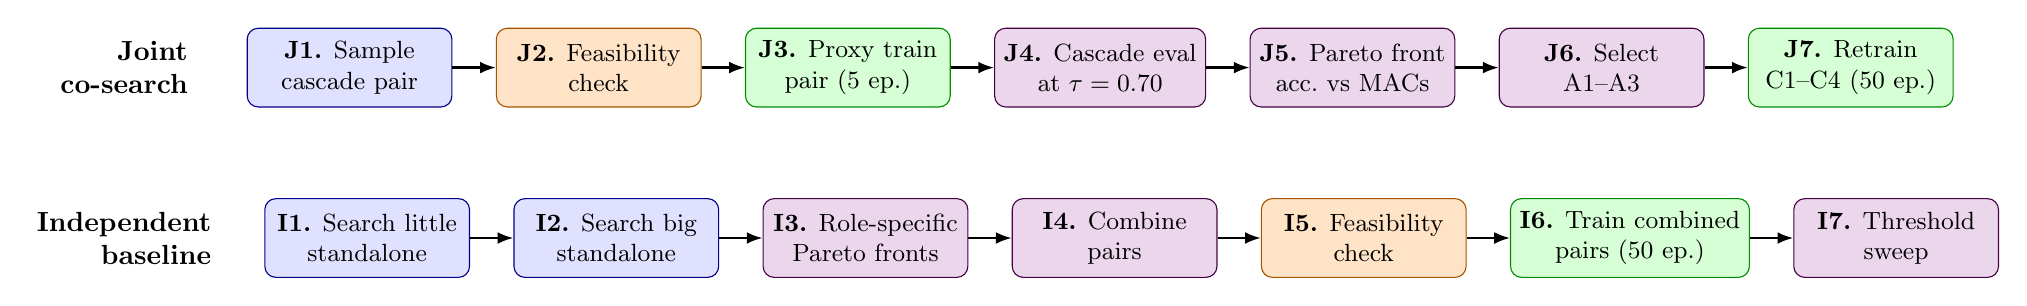
\begin{tikzpicture}[
    node distance=0.85cm and 0.55cm,
    stage/.style={
        draw,
        rounded corners,
        align=center,
        minimum width=2.6cm,
        minimum height=1.0cm,
        font=\small
    },
    sample/.style={stage, fill=blue!12, draw=blue!55!black},
    check/.style={stage, fill=orange!22, draw=orange!65!black},
    train/.style={stage, fill=green!16, draw=green!55!black},
    eval/.style={stage, fill=violet!16, draw=violet!55!black},
    labelbox/.style={
        align=right,
        font=\bfseries,
        minimum width=2.0cm
    },
    arrow/.style={-{Latex[length=2mm]}, thick}
]
\node[labelbox] (jointlabel) {Joint\\co-search};
\node[sample, right=of jointlabel] (jsample) {\textbf{J1.} Sample\\cascade pair};
\node[check, right=of jsample] (jcheck) {\textbf{J2.} Feasibility\\check};
\node[train, right=of jcheck] (jproxy) {\textbf{J3.} Proxy train\\pair (5 ep.)};
\node[eval, right=of jproxy] (jeval) {\textbf{J4.} Cascade eval\\at $\tau=0.70$};
\node[eval, right=of jeval] (jfront) {\textbf{J5.} Pareto front\\acc.\ vs MACs};
\node[eval, right=of jfront] (jselect) {\textbf{J6.} Select\\A1--A3};
\node[train, right=of jselect] (jretrain) {\textbf{J7.} Retrain\\C1--C4 (50 ep.)};

\node[labelbox, below=1.25cm of jointlabel] (indlabel) {Independent\\baseline};
\node[sample, right=of indlabel] (isample) {\textbf{I1.} Search little\\standalone};
\node[sample, right=of isample] (isampleb) {\textbf{I2.} Search big\\standalone};
\node[eval, right=of isampleb] (ifronts) {\textbf{I3.} Role-specific\\Pareto fronts};
\node[eval, right=of ifronts] (icombine) {\textbf{I4.} Combine\\pairs};
\node[check, right=of icombine] (icheck) {\textbf{I5.} Feasibility\\check};
\node[train, right=of icheck] (itrain) {\textbf{I6.} Train combined\\pairs (50 ep.)};
\node[eval, right=of itrain] (isweep) {\textbf{I7.} Threshold\\sweep};

\draw[arrow] (jsample) -- (jcheck);
\draw[arrow] (jcheck) -- (jproxy);
\draw[arrow] (jproxy) -- (jeval);
\draw[arrow] (jeval) -- (jfront);
\draw[arrow] (jfront) -- (jselect);
\draw[arrow] (jselect) -- (jretrain);

\draw[arrow] (isample) -- (isampleb);
\draw[arrow] (isampleb) -- (ifronts);
\draw[arrow] (ifronts) -- (icombine);
\draw[arrow] (icombine) -- (icheck);
\draw[arrow] (icheck) -- (itrain);
\draw[arrow] (itrain) -- (isweep);
\end{tikzpicture}%
}
\caption{Joint co-search pipeline (top, J1-J7) versus the independent NAS
baseline (bottom, I1-I7). Stages are coloured by type: blue = sample /
search, orange = feasibility filter, green = training (proxy or final),
violet = evaluation, frontier, and selection. The joint pipeline sees the
cascade as a coupled object from J3 onward, whereas the independent
baseline does not assemble cascade pairs until I4. The text in
Sections~\ref{sec:methodology:joint} and~\ref{sec:methodology:baseline}
refers to these step labels.}
\label{fig:search-pipeline}
\end{figure*}

\subsection{Cascade-Aware Loss}
\label{sec:methodology:loss}

We use a cascade-aware retraining loss that keeps standard classification
terms but reflects how the cascade routes samples at inference time. We use
\emph{co-training} in the sense of jointly optimising the little and big
models with a shared loss, which is unrelated to semi-supervised
co-training.
The hard routing decision (Eq.~\ref{eq:max-softmax}) is replaced during
training by a differentiable soft exit probability
\begin{equation}
p_{\mathrm{exit}} = \sigma\bigl(k\,(c_l-\tau)\bigr),
\label{eq:soft-exit}
\end{equation}
where $\sigma$ is the sigmoid function and $k$ is a routing sharpness
parameter. Large $k$ makes the soft decision approach the hard threshold
rule, while small $k$ smooths it out. We use $k=20$, which gives
$p_{\mathrm{exit}}\approx 1$ for $c_l\gtrsim 0.85$ and $p_{\mathrm{exit}}
\approx 0$ for $c_l\lesssim 0.55$ at $\tau=0.70$; this is sharp enough to
behave like the inference-time threshold for most samples while keeping a
small interval of gradient flow around $\tau$.

\begin{figure}[t]
\centering
\resizebox{\columnwidth}{!}{%
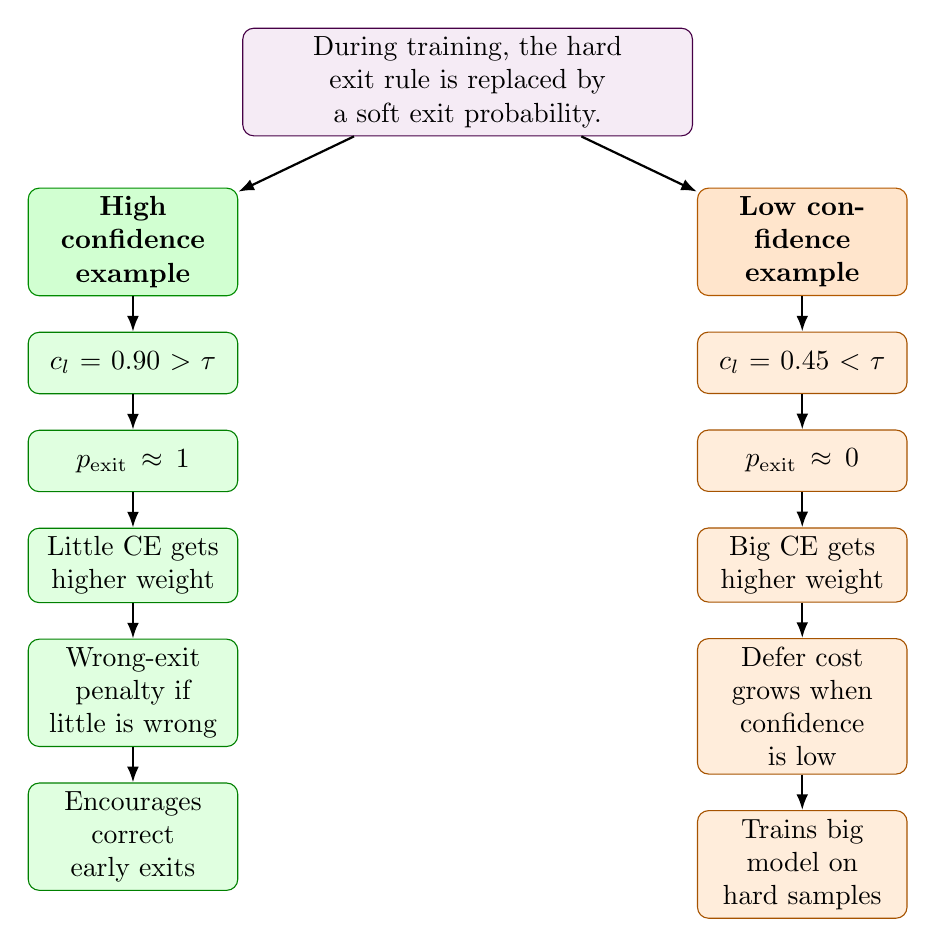
\begin{tikzpicture}[
    node distance=0.45cm and 0.45cm,
    box/.style={
        draw,
        rounded corners,
        align=center,
        text width=2.45cm,
        minimum height=0.78cm,
        inner sep=3pt
    },
    context/.style={box, fill=violet!8, draw=violet!55!black},
    highbox/.style={box, fill=green!12, draw=green!50!black},
    lowbox/.style={box, fill=orange!14, draw=orange!65!black},
    header/.style={
        draw,
        rounded corners,
        align=center,
        font=\bfseries,
        text width=2.45cm,
        minimum height=0.75cm,
        inner sep=3pt
    },
    highheader/.style={header, fill=green!18, draw=green!55!black},
    lowheader/.style={header, fill=orange!20, draw=orange!70!black},
    arrow/.style={-{Latex[length=2mm]}, thick}
]
\node[context, text width=5.5cm] (batch) {During training, the hard exit rule is replaced by a soft exit probability.};
\node[highheader, below left=0.65cm and 0.05cm of batch] (highh) {High confidence\\example};
\node[lowheader, below right=0.65cm and 0.05cm of batch] (lowh) {Low confidence\\example};

\node[highbox, below=of highh] (highc) {$c_l=0.90>\tau$};
\node[lowbox, below=of lowh] (lowc) {$c_l=0.45<\tau$};
\node[highbox, below=of highc] (highp) {$p_{\mathrm{exit}}\approx 1$};
\node[lowbox, below=of lowc] (lowp) {$p_{\mathrm{exit}}\approx 0$};
\node[highbox, below=of highp] (highloss) {Little CE gets higher weight};
\node[lowbox, below=of lowp] (lowloss) {Big CE gets higher weight};
\node[highbox, below=of highloss] (highpen) {Wrong-exit penalty if little is wrong};
\node[lowbox, below=of lowloss] (lowpen) {Defer cost grows when confidence is low};
\node[highbox, below=of highpen] (higheffect) {Encourages correct early exits};
\node[lowbox, below=of lowpen] (loweffect) {Trains big model on hard samples};

\draw[arrow] (batch) -- (highh);
\draw[arrow] (batch) -- (lowh);
\draw[arrow] (highh) -- (highc);
\draw[arrow] (lowh) -- (lowc);
\draw[arrow] (highc) -- (highp);
\draw[arrow] (lowc) -- (lowp);
\draw[arrow] (highp) -- (highloss);
\draw[arrow] (lowp) -- (lowloss);
\draw[arrow] (highloss) -- (highpen);
\draw[arrow] (lowloss) -- (lowpen);
\draw[arrow] (highpen) -- (higheffect);
\draw[arrow] (lowpen) -- (loweffect);
\end{tikzpicture}%
}
\caption{Behavioral view of the cascade-aware loss. Green shows the
high-confidence path, where samples are treated as likely early exits; orange
shows the low-confidence path, where samples are treated as likely deferrals.
The soft exit probability shifts the learning emphasis between the little and
big models.}
\label{fig:cotraining-loss-flow}
\end{figure}

The full cascade-aware loss has four terms:
\begin{equation}
\begin{aligned}
\mathcal{L}_{\mathrm{cascade}}
={}& \underbrace{(p_{\mathrm{exit}}+\lambda_l)\,\mathrm{CE}(z_l,y)}_{\text{little CE, routed}} \\
&+ \underbrace{(1-p_{\mathrm{exit}}+\lambda_b)\,\mathrm{CE}(z_b,y)}_{\text{big CE, routed}} \\
&+ \underbrace{\lambda_d\,(1-p_{\mathrm{exit}})}_{\text{defer cost}}
+ \underbrace{\lambda_w\,p_{\mathrm{exit}}\,\mathbf{1}[\hat{y}_l \neq y]}_{\text{wrong-exit penalty}}.
\end{aligned}
\label{eq:cascade-loss}
\end{equation}
The first two CE terms emphasise the little (resp.\ big) model on samples
likely to exit (resp.\ defer); the constants $\lambda_l$ and $\lambda_b$
keep a small training signal flowing to both models even when the soft
routing weight is near zero. The third term is a small defer cost that
prevents the optimiser from sending every sample to the big model, which
would maximise accuracy but eliminate the cascade's compute saving. The
fourth term penalises confident wrong exits, the failure mode that
directly hurts a threshold-routed cascade. The routing-related terms are
deliberately small relative to the CE terms. Large values dominate the
classification objective and produce miscalibrated branches.
Figure~\ref{fig:cotraining-loss-flow} illustrates these effects for
high-confidence and low-confidence samples.

We use $\lambda_l=0.75$, $\lambda_b=0.05$, $\lambda_d=0.0125$, and
$\lambda_w=0.075$ throughout. These values were selected by manual
calibration on the CIFAR-10 validation split rather than by a full sweep:
$\lambda_l$ is the largest so that the little branch always receives a
classification signal; $\lambda_b$ is smaller because the big branch is
mostly trained on deferred samples already; $\lambda_d$ and $\lambda_w$ are
small enough to act as routing-aware regularisers without dominating the CE
terms. A systematic sensitivity sweep is left to future work
(\S\ref{sec:future-work}).

\subsection{Retraining Loss Ablations}
\label{sec:methodology:loss-ablations}

For RQ2, the three selected joint-NAS architectures are retrained from
scratch under the four loss settings of
Table~\ref{tab:retraining-loss-ablations}. The ablation isolates whether
improvements come from standard cross-entropy (C1), label smoothing (C2),
the cascade-aware loss (C3), or its combination with label smoothing (C4).
CE is the default baseline because it is the standard supervised
classification objective \cite{goodfellow2016deeplearning}.
Label smoothing is included because cascade routing depends on confidence,
and smoothing is a simple calibration-oriented baseline
\cite{mueller2019labelsmoothing,guo2017calibration}.

\begin{table}[H]
\centering
\caption{Retraining loss ablations.}
\label{tab:retraining-loss-ablations}
\begin{tabular}{ll}
\toprule
\textbf{Condition} & \textbf{Retraining loss} \\
\midrule
C1 & Cross-entropy (CE) \\
C2 & CE + label smoothing \\
C3 & Cascade-aware loss \\
C4 & Cascade-aware loss + label smoothing \\
\bottomrule
\end{tabular}
\end{table}

% ============================================================================
\section{Experimental Setup}
\label{sec:experiments}

\subsection{Datasets}

All experiments use CIFAR-10 \cite{krizhevsky2009cifar}, a 10-class
$32\times 32$ image classification dataset with 50K training and 10K test
images. We use a deterministic 45K/5K split of the training set: approximately 500 images
per class (Figure \ref{fig:cifar10_validation_split}) are held out for validation and the remaining 45K are used for
training. Table~\ref{tab:retraining-loss-ablations};
\begin{figure}[t]
\centering
\resizebox{\columnwidth}{!}{%
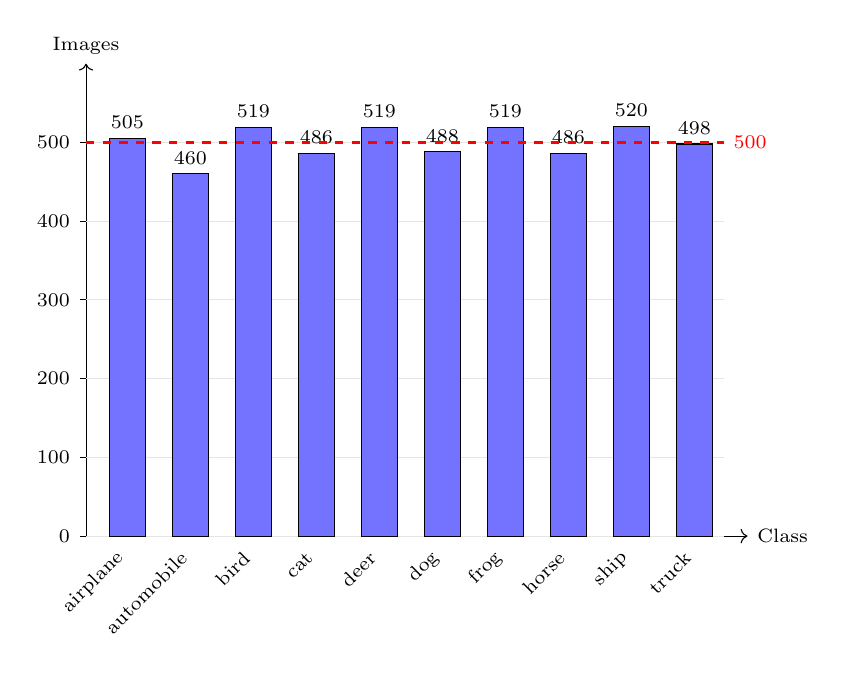
\begin{tikzpicture}
    % Axes
    \draw[->] (0,0) -- (8.4,0) node[right] {\scriptsize Class};
    \draw[->] (0,0) -- (0,6.0) node[above] {\scriptsize Images};

    % Y-axis ticks
    \foreach \y in {0,100,200,300,400,500} {
        \pgfmathsetmacro{\yy}{\y/100}
        \draw (-0.08,\yy) -- (0,\yy);
        \node[left, font=\scriptsize] at (-0.08,\yy) {\y};
        \draw[gray!20] (0,\yy) -- (8.1,\yy);
    }

    % Bars: class / count / x-position
    \foreach \cls/\n/\x in {
        airplane/505/0.3,
        automobile/460/1.1,
        bird/519/1.9,
        cat/486/2.7,
        deer/519/3.5,
        dog/488/4.3,
        frog/519/5.1,
        horse/486/5.9,
        ship/520/6.7,
        truck/498/7.5
    } {
        \pgfmathsetmacro{\h}{\n/100}
        \draw[fill=blue!55, draw=black] (\x,0) rectangle ++(0.45,\h);
        \node[above, font=\scriptsize] at (\x+0.225,\h) {\n};
        \node[rotate=45, anchor=east, font=\scriptsize] at (\x+0.225,-0.15) {\cls};
    }

    % Ideal balanced reference line
    \draw[red, dashed, thick] (0,5.0) -- (8.1,5.0);
    \node[right, red, font=\scriptsize] at (8.1,5.0) {500};
\end{tikzpicture}%
}
\caption{Class distribution of the first 5,000 CIFAR-10 training images used as the validation split.}
\label{fig:cifar10_validation_split}
\end{figure}

The official 10K test split is kept untouched and used only for
the final threshold-sweep evaluation. CIFAR-10 is small enough to support
repeated NAS proxy training and ablation runs while remaining non-trivial
for confidence-based routing and calibration analysis. Training uses
random crop with 4-pixel padding and random horizontal flipping, followed
by CIFAR-10 normalisation; validation and test use the same normalisation
without augmentation.

\subsection{Training Schedule}

The training schedule is summarised in Table~\ref{tab:experimental-schedule}.
The joint search uses a population of 20 for 20 generations; the independent
baseline uses 20 for 10 generations \emph{per role}, since it runs one
little-model and one big-model search sequentially. This gives the two
methods approximately the same number of proxy-trained candidates (the
quantity that dominates compute cost), even though the evolutionary depth
per role differs. The independent baseline does not use the cascade-aware
shared loss: it trains the selected little and big architectures as
standalone CE classifiers, and the two are coupled only at evaluation via
the threshold router.

Retraining starts from scratch under each of the four C1-C4 conditions in
Table~\ref{tab:retraining-loss-ablations}; proxy-trained weights are not
re-used. The 50-epoch retraining budget is the longest schedule we could
afford across all variants given the total compute budget. Many CIFAR-style
setups train for 100-200 epochs; we discuss the implications of the
shorter schedule in Section~\ref{sec:future-work}.

\begin{table}[t]
\centering
\caption{Training and evaluation schedule used in the experiments.}
\label{tab:experimental-schedule}
\small
\begin{tabular}{@{}p{0.30\columnwidth}p{0.34\columnwidth}p{0.24\columnwidth}@{}}
\toprule
\textbf{Stage} & \textbf{Setting} & \textbf{Value} \\
\midrule
Joint NAS & Population / generations & 20 / 20 \\
Independent NAS & Population / generations & 20 / 10 per role \\
Proxy training & Epochs / batch size & 5 / 128 \\
Proxy training & Optimizer & SGD, lr 0.05 \\
Joint C1-C4 retraining & Epochs / batch size & 50 / 128 \\
Joint C1-C4 retraining & Optimizer & SGD, lr 0.1 \\
Joint C1-C4 retraining & Scheduler & Cosine annealing \cite{loshchilov2017sgdr} \\
Independent final training & Epochs / learning rate & 50 / 0.05 \\
All final training & Momentum / weight decay & 0.9 / $5\cdot10^{-4}$ \\
Threshold sweep & Thresholds & 0.50, 0.60, 0.70, 0.80, 0.90, 0.95 \\
\bottomrule
\end{tabular}
\end{table}

\subsection{Evaluation Metrics}

The primary metrics are cascade accuracy and expected cascade MACs (the cost
model defined in Eq.~\ref{eq:cascade-cost}). Secondary metrics are the exit
ratio $\rho$, the standalone little- and big-model accuracies, parameter
count, and the float32 deployment-memory estimate (both models' weights plus
the input buffer plus the larger of the two peak activation footprints,
since the two models are evaluated sequentially). All analytical metrics
support NAS selection and the main accuracy-compute comparisons.
Measured Pico 2 latency and TFLM arena sizes are reported separately
(Section~\ref{sec:results:pico}).

For routing and calibration we report the little-model ECE
(Section~\ref{sec:background:ece}) and the \emph{routing error rate}, the
fraction of test samples on which the cascade exits at the little model with
a wrong prediction even though the big model would have been correct. This
captures the failure mode that directly hurts a threshold-routed cascade.
Proxy-search and final-retrained results are reported separately: proxy
metrics are 5-epoch validation accuracies used only for architecture
selection, whereas final claims use 50-epoch retrained test-set
threshold-sweep results.

\subsection{Implementation Details}

All experiments are implemented in PyTorch through a scripted pipeline that
runs joint NAS, independent NAS, retraining, metric aggregation, and plot
generation. CUDA is used when available, CPU otherwise. All experiments use
random seed 42, which is propagated to Python, NumPy, PyTorch, CUDA, the
NSGA-II implementation, feasible-sampling and repair operators, and
DataLoader shuffling. Experiment outputs are saved as CSV files, including search logs, Pareto fronts, selected architectures, training curves, and threshold sweeps. The reported results tables and figures are generated from these files, allowing the results to be recomputed without retraining.

\subsection{Pico 2 Deployment Test Setup}

After final retraining, the selected cascades were exported to ONNX and then to
float32 TensorFlow Lite models for TensorFlow Lite Micro. The exported little
and big models were converted into C arrays and compiled into Raspberry Pi Pico
2 firmware. The Pico firmware implements the same threshold router used in the
offline evaluation: each image is first evaluated by the little model, the
maximum softmax confidence is compared with $\tau=0.70$, and only
low-confidence samples are deferred to the big model.

Two Pico experiments were run. First, the normal latency and accuracy test used
a USB serial protocol in which the host streamed CIFAR-10 test images to the
Pico one sample at a time. This allowed the full 10,000-image CIFAR-10 test set
to be evaluated without storing the entire dataset in Pico flash. For each
sample, the Pico reported the predicted class, route decision, correctness,
little-model time, big-model time when used, total cascade time, and analytical
MAC counts for the selected path. This is the source of the deployment latency
and route-split results reported in Table~\ref{tab:pico-deployment}.

Second, a route-aware energy test was run on a 1,000-image embedded CIFAR-10
subset. This version stores the test subset in Pico flash and runs without USB
power during measurement. Figure~\ref{fig:pico-energy-setup} shows the
measurement circuit. An Elegoo Uno R3 powers the Pico 2 through a 10~$\Omega$
high-side shunt connected to VSYS. The Uno samples the voltage before and after
the shunt to estimate current and power, while Pico GP18 drives an inference
trigger connected to Uno D2. In the route-aware build, Pico GP19 also indicates
the route decision to Uno D3, with the high state representing deferred
big-model execution. This setup separates idle time from the active inference
window and records whether each measured inference used the little path or the
deferred path.

\begin{figure*}[t]
\centering
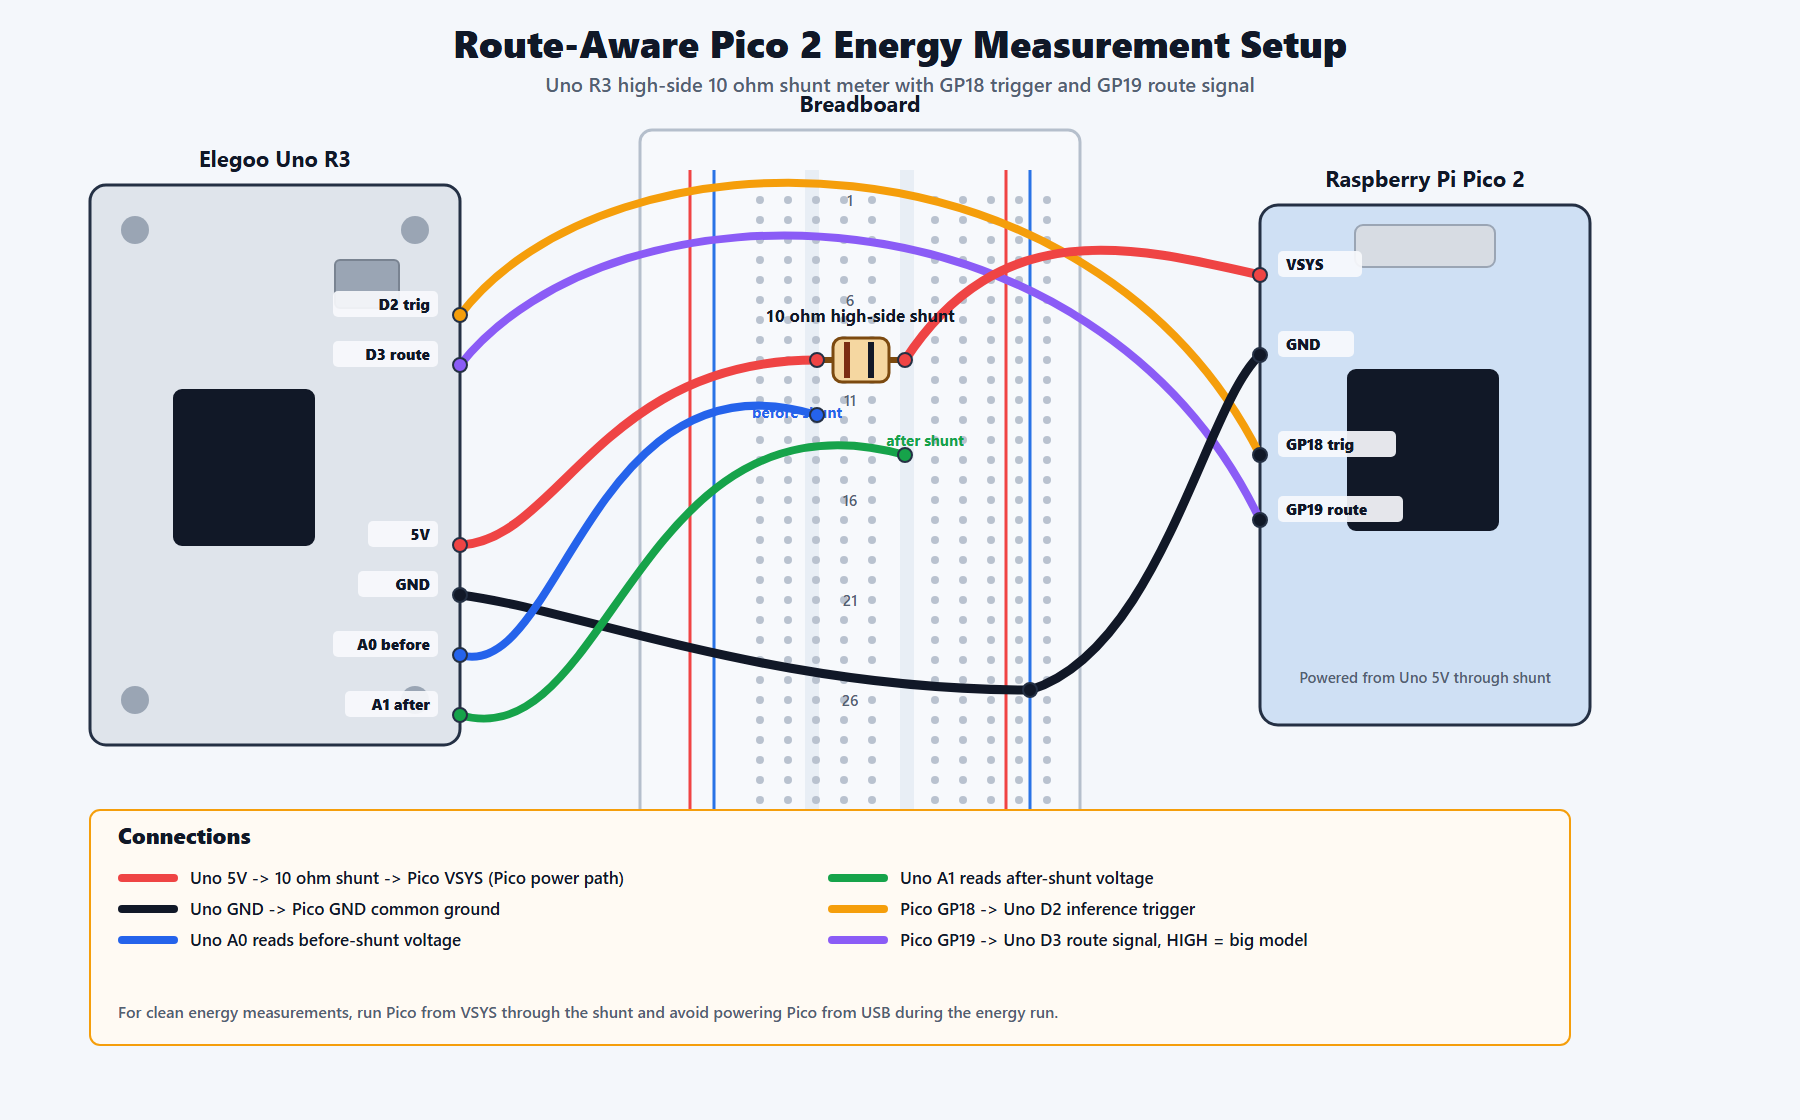
\includegraphics[width=0.90\textwidth]{pico_uno_energy_fritzing_diagram.png}
\caption{Route-aware Pico 2 energy measurement setup using a 10~$\Omega$
high-side shunt, GP18 inference trigger, and GP19 route signal.}
\label{fig:pico-energy-setup}
\end{figure*}

% ============================================================================

\section{Results}
\label{sec:results}

All reported results in this section use the final retrained checkpoints and
the CIFAR-10 test split. Unless otherwise stated, results are reported at the
fixed operating threshold $\tau=0.70$, matching the main comparison used in
the generated figures.

\subsection{RQ1: Joint Co-Search vs.\ Independent NAS}

Table~\ref{tab:rq1-results} summarizes the final joint and independent cascade
results. The joint co-search pipeline occupies a stronger accuracy-MACs
region than the independent baseline. C3 is the cheaper cascade-aware variant, reaching
79.69\% mean test accuracy at 1.67M average cascade MACs, while C4 reaches the
highest mean accuracy, 80.69\%, at a higher 2.08M average cascade MACs. The
independent baseline reaches 74.03\% at 2.22M average cascade MACs. Thus, at
the fixed threshold used for the main comparison, the joint variants provide
substantially higher accuracy, and the cheaper C3 operating point also uses
less expected compute than the independent baseline.

\begin{table}[t]
\centering
\caption{RQ1 test-set comparison at $\tau=0.70$. Values are averaged across the
three selected retrained cascades. C1-C4 share the same co-searched
architectures but differ in retraining loss. The independent baseline is
searched and combined separately. ECE is Expected Calibration Error
(\S\ref{sec:background}); lower is better.}
\label{tab:rq1-results}
\footnotesize
\begin{tabular}{@{}lrrrr@{}}
\toprule
\textbf{Method}      & \textbf{Acc.\ (\%)} & \textbf{Exit ratio} & \textbf{MACs (M)} & \textbf{ECE} \\
\midrule
Joint NAS C1         & 79.64 & 0.55 & 1.69 & 0.0104 \\
Joint NAS C2         & 80.33 & 0.43 & 2.01 & 0.0811 \\
Joint NAS C3         & 79.69 & 0.55 & 1.67 & 0.0104 \\
Joint NAS C4         & 80.69 & 0.40 & 2.08 & 0.0850 \\
Independent NAS      & 74.03 & 0.57 & 2.22 & 0.0508 \\
\bottomrule
\end{tabular}
\end{table}

The individual C4 cascades range from 79.77\% to 81.71\% accuracy at
$\tau=0.70$, while the independent cascades range from 72.67\% to 75.96\%.
C3 gives a lower-compute joint operating point with similar accuracy to C1,
whereas C4 gives the high-accuracy, high-deferral end of the ablation. This
indicates that the joint pipeline is stronger than the independent baseline,
but that the final operating point still depends on the retraining objective.
The high-accuracy joint comparison is visualized in
Figure~\ref{fig:rq1-joint-independent}.

\begin{figure*}[t]
\centering

\includegraphics[width=0.92\textwidth]{joint_vs_independent_size_compute.pdf}
\caption{Final retrained high-accuracy joint cascades compared with
independently searched cascades at the fixed operating threshold $\tau=0.70$.
The plot uses the C4 retraining condition to show the high-accuracy end of the
joint ablation, not to define C4 as the single canonical joint result. The left
panel compares combined parameter count against cascade accuracy, while the
right panel compares expected cascade MACs against cascade accuracy.}
\label{fig:rq1-joint-independent}
\end{figure*}

\subsection{RQ2: CE vs.\ Cascade-Aware Retraining}

Table~\ref{tab:rq2-results} reports the retraining-loss ablation for the same
three joint-NAS architectures. C1 and C3 compare CE against the cascade-aware
loss without label smoothing. Their average cascade accuracies are close, but
C3 slightly improves over C1 while also reducing expected MACs: C1 obtains
79.64\% at 1.69M MACs, while C3 obtains 79.69\% at 1.67M MACs. This is not a
large standalone win, but it shows that the cascade-aware loss can move the
operating point in the intended direction.

\begin{table}[t]
\centering
\caption{RQ2 retraining-loss ablation at $\tau=0.70$. Values are averaged over
the three selected joint architectures (A1, A2, A3).}
\label{tab:rq2-results}
\scriptsize
\setlength{\tabcolsep}{4pt}
\begin{tabular}{@{}lrrrr@{}}
\toprule
\textbf{Variant}          & \textbf{Acc.\ (\%)} & \textbf{Exit} & \textbf{MACs} & \textbf{Route err.} \\
                          &                     & \textbf{ratio} & \textbf{(M)}  &                    \\
\midrule
C1: CE                    & 79.64 & 0.55 & 1.69 & 0.0231 \\
C2: CE + smooth           & 80.33 & 0.43 & 2.01 & 0.0093 \\
C3: Cascade loss          & 79.69 & 0.55 & 1.67 & 0.0242 \\
C4: Cascade + smooth      & 80.69 & 0.40 & 2.08 & 0.0083 \\
\bottomrule
\end{tabular}
\end{table}

The smoothed variants, C2 and C4, achieve the highest average cascade
accuracies. They also have substantially lower routing error rates than C1 and
C3, but this comes with lower exit ratios and therefore higher expected
cascade MACs. The ablation itself thus shows an accuracy-compute trade-off: C1 and C3 exit more often and are cheaper, while C2 and C4
defer more samples and obtain higher accuracy. C4 is the higher-accuracy,
higher-compute variant; C3 is the cheaper cascade-aware alternative. These trends are shown in
Figure~\ref{fig:rq2-ablation}.

\begin{figure}[t]
\centering

\includegraphics[width=\columnwidth]{ablation_acc_vs_flops.pdf}
\caption{Retraining-loss ablation for the three selected joint
architectures at $\tau=0.70$, plotted in the accuracy-MACs plane. C1 uses
CE, C2 uses CE with label smoothing, C3 uses the cascade-aware loss, and
C4 combines cascade-aware loss with label smoothing. C3 marginally
improves on the CE operating point of C1; the smoothed variants (C2, C4)
sit higher on accuracy but also use more MACs because they defer more
often.}
\label{fig:rq2-ablation}
\end{figure}

\subsection{Routing Behaviour and Threshold Sensitivity}
\label{sec:results:routing}

The two research questions concern \emph{which} architecture and \emph{which}
loss to use at a single operating threshold. This subsection complements
them by examining \emph{how} the selected joint cascades behave at the
operating threshold and across a sweep of alternative thresholds.

At $\tau=0.70$, the routing-error rate of the C4 variant is 0.0083, against
0.0231 and 0.0242 for C1 and C3 respectively (Table~\ref{tab:rq2-results}).
The highest-accuracy variant also makes the fewest harmful early-exit
decisions. ECE and routing error do not, however, move together:
C1 and C3 have the lowest little-model ECE but the highest routing error.
Global calibration is necessary but not sufficient to explain cascade
quality. What matters for the threshold router is whether
\emph{high-confidence} little predictions are correct on the samples that
actually exit. Figure~\ref{fig:routing-diagnostics} shows this relationship.

\begin{figure*}[t]
\centering
\begin{minipage}{0.48\textwidth}
    \centering
    
\includegraphics[width=\linewidth]{ablation_ece_routing_at_070.pdf}
\end{minipage}
\hfill
\begin{minipage}{0.48\textwidth}
    \centering
    
\includegraphics[width=\linewidth]{accuracy_vs_exit_ratio.pdf}
\end{minipage}
\caption{Routing and confidence behaviour at $\tau=0.70$. \emph{Left:}
little-model ECE and routing error for C1-C4. \emph{Right:} cascade
accuracy vs.\ early-exit ratio for joint and independent cascades. Exit
ratio alone does not predict cascade quality: it must be read alongside
routing error and confidence calibration.}
\label{fig:routing-diagnostics}
\end{figure*}

The threshold $\tau=0.70$ is one operating point on a continuum.
Figure~\ref{fig:threshold-sensitivity} sweeps $\tau$ from 0.50 to 0.95
for C1-C4. Lower thresholds produce cheaper, more exit-heavy cascades;
higher thresholds approach big-model behaviour. The cascade-aware variants
(C3 and C4) were trained with $\tau=0.70$ embedded in the soft routing
term, and remain competitive across mid thresholds, but lose their edge
once $\tau$ is pushed well above the training value.

\begin{figure*}[t]
\centering

\includegraphics[width=0.92\textwidth]{ablation_threshold_sweep_acc_exit.pdf}
\caption{Threshold sweep for C1-C4. Increasing $\tau$ reduces the exit
ratio and generally improves accuracy by deferring more samples to the big
model.}
\label{fig:threshold-sensitivity}
\end{figure*}

\subsection{Pico 2 Deployment Results}
\label{sec:results:pico}

To check whether the analytical cascade metrics transfer to an embedded target,
the selected A2 C1-C4 cascades were exported from PyTorch checkpoints to
ONNX and float32 TensorFlow Lite Micro models, then compiled into Raspberry Pi
Pico 2 firmware. The independent NAS genotype 4 baseline was exported through
the same path. The normal deployment test streamed the full CIFAR-10 test set
over USB serial, so each operating point was evaluated on 10,000 images. All
Pico runs used the same confidence threshold $\tau=0.70$ as the main
comparison and the same softmax
defined in Section~\ref{sec:background:routing}.

\begin{table*}[t]
\centering
\caption{Pico 2 serial CIFAR-10 deployment results at $\tau=0.70$.
\textbf{Exit} and \textbf{Defer} report the percentage of the 10{,}000 test
samples that the threshold router exited at the little model and deferred to
the big model respectively. \textbf{Little ms} is the end-to-end latency for
samples that exit after the little model; \textbf{Defer ms} includes the
little plus the big model.}
\label{tab:pico-deployment}
\small
\begin{tabular}{@{}lrrrrrr@{}}
\toprule
\textbf{Cascade} & \textbf{Acc.\ (\%)} & \textbf{Exit (\%)} & \textbf{Defer (\%)} &
\textbf{Little (ms)} & \textbf{Defer (ms)} & \textbf{Avg (ms)} \\
\midrule
A2 C1            & 78.97 & 42.86 & 57.14 & 40.34 & 204.19 & 133.97 \\
A2 C2            & 79.96 & 32.66 & 67.34 & 40.36 & 204.21 & 150.70 \\
A2 C3            & 78.94 & 42.64 & 57.36 & 40.34 & 204.20 & 134.33 \\
A2 C4            & 80.46 & 27.60 & 72.40 & 40.37 & 204.22 & 159.00 \\
Independent 4    & 73.47 & 58.99 & 41.01 & 131.93 & 848.45 & 425.77 \\
\bottomrule
\end{tabular}
\end{table*}

The A2 variants have almost identical per-path latency because they share
the same exported architecture and differ mainly in trained weights and routing
behaviour. Their little path takes about 40.3 ms, while a deferred sample takes
about 204.2 ms end-to-end. The average latency therefore follows the observed
route split: C1 and C3 are the fastest A2 variants because they exit on
about 43\% of the test set, whereas C4 reaches the highest Pico accuracy but
defers 72.4\% of samples and is correspondingly slower. The independent
baseline exits more often than any A2 variant, but its little and deferred
paths are much slower, giving a much higher average latency despite its higher
exit ratio.

The deployment also exposed a memory distinction that is not visible from
accuracy and MACs alone. The A2 firmware used separate TensorFlow Lite
Micro arenas of 128 KiB for the little model and 256 KiB for the big model,
while the independent firmware required arena tuning and was finally tested
with a 96 KiB little arena and a 352 KiB big arena. Additional independent
energy builds with 160/288, 192/256, 224/224, and 256/192 KiB arena splits
were produced to diagnose feasible allocations. This suggests that practical
deployment feasibility depends not only on model weights and analytical MACs,
but also on activation memory and TensorFlow Lite Micro arena requirements.

\subsection{Energy Consumption}

In addition to latency, a smaller route-aware energy experiment was run to
measure whether the deployed cascade behaviour translates into lower energy
use. Unlike the normal serial test, this energy run used a 1,000-image CIFAR-10
subset embedded directly in Pico flash. This avoided USB streaming during the
measurement window and allowed the Pico to be powered through the Uno/shunt
path shown in Figure~\ref{fig:pico-energy-setup}. The Pico raised GP18 only
during active cascade inference, so the Uno measurement excluded most idle
time. The route-aware build also used GP19 to indicate whether a sample
deferred to the big model.

\begin{table*}[t]
\centering
\caption{Route-aware Pico 2 energy measurement on a 1{,}000-sample embedded
CIFAR-10 subset. \textbf{Joint A2 (C4)} is the high-accuracy
cascade-aware + label-smoothing variant of the co-searched A2 cascade used
for the deployment comparison. \textbf{Exit} and \textbf{Defer} are the
percentage of the 1{,}000 samples handled by the little path and the
deferred path respectively.}
\label{tab:pico-energy}
\small
\begin{tabular}{@{}lrrrrrr@{}}
\toprule
\textbf{Cascade}  & \textbf{Time (s)} & \textbf{Energy (J)} &
\textbf{J/sample} & \textbf{Power (W)} & \textbf{Exit (\%)} & \textbf{Defer (\%)} \\
\midrule
Independent 4     & 428.7 & 44.0 & 0.044 & 0.099 & 58.5 & 41.5 \\
Joint A2 (C4)     & 330.1 & 34.3 & 0.034 & 0.105 & 53.0 & 47.0 \\
\bottomrule
\end{tabular}
\end{table*}

The joint A2 cascade used 34.3 J over the embedded subset, compared with
44.0 J for the independent baseline. This is a 22.0\% reduction in total energy
and approximately the same reduction per image. Runtime also decreased from
428.7 s to 330.1 s, a 23.0\% reduction. The average measured power is similar
between the two runs, and is slightly higher for the joint cascade, so the
energy saving is mainly explained by the shorter active inference time rather
than by a lower instantaneous power draw.

\begin{figure}[t]
\centering
\resizebox{\columnwidth}{!}{%
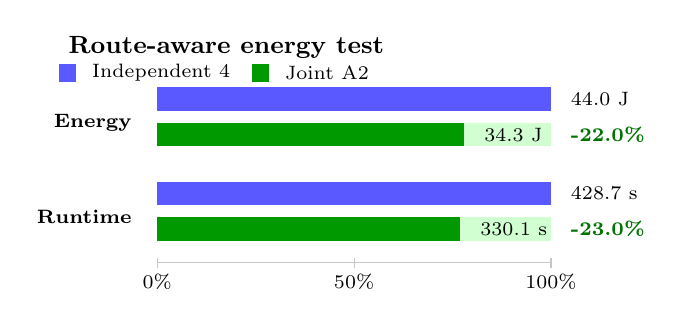
\begin{tikzpicture}[x=1cm,y=1cm]
    \node[font=\small\bfseries, anchor=west] at (0,3.15)
        {Route-aware energy test};
    \fill[blue!65] (0,2.72) rectangle (0.22,2.94);
    \node[anchor=west] at (0.30,2.83) {\scriptsize Independent 4};
    \fill[green!60!black] (2.45,2.72) rectangle (2.67,2.94);
    \node[anchor=west] at (2.75,2.83) {\scriptsize Joint A2};

    \node[anchor=east, font=\scriptsize\bfseries] at (1.05,2.20) {Energy};
    \fill[blue!18] (1.25,2.35) rectangle (6.25,2.65);
    \fill[blue!65] (1.25,2.35) rectangle (6.25,2.65);
    \node[anchor=west] at (6.38,2.50) {\scriptsize 44.0 J};
    \fill[green!18] (1.25,1.90) rectangle (6.25,2.20);
    \fill[green!60!black] (1.25,1.90) rectangle (5.15,2.20);
    \node[anchor=west] at (5.28,2.05) {\scriptsize 34.3 J};
    \node[anchor=west, font=\scriptsize\bfseries, green!45!black]
        at (6.38,2.05) {-22.0\%};

    \node[anchor=east, font=\scriptsize\bfseries] at (1.05,1.00) {Runtime};
    \fill[blue!18] (1.25,1.15) rectangle (6.25,1.45);
    \fill[blue!65] (1.25,1.15) rectangle (6.25,1.45);
    \node[anchor=west] at (6.38,1.30) {\scriptsize 428.7 s};
    \fill[green!18] (1.25,0.70) rectangle (6.25,1.00);
    \fill[green!60!black] (1.25,0.70) rectangle (5.10,1.00);
    \node[anchor=west] at (5.23,0.85) {\scriptsize 330.1 s};
    \node[anchor=west, font=\scriptsize\bfseries, green!45!black]
        at (6.38,0.85) {-23.0\%};

    \draw[gray!45] (1.25,0.42) -- (6.25,0.42);
    \foreach \x/\label in {1.25/0,3.75/50,6.25/100}
        \draw[gray!45] (\x,0.36) -- (\x,0.48)
            node[below=0.08cm, black] {\scriptsize \label\%};
\end{tikzpicture}}
\caption{Normalized route-aware Pico 2 energy-test comparison. Independent 4
is shown as the 100\% baseline; the joint A2 cascade reduces total energy by
22.0\% and runtime by 23.0\% on the 1,000-sample embedded subset.}
\label{fig:pico-energy-comparison}
\end{figure}

The route counts make this result especially useful. In the energy run, the
joint cascade actually deferred slightly more samples than the independent
baseline, but still consumed less total energy. This matches the latency result
in Table~\ref{tab:pico-deployment}: the joint A2 paths are substantially
faster, so the energy benefit does not come only from exiting more often. It
comes from the deployed cost of each path. The independent baseline has a high
exit ratio, but its little path and deferred path are both expensive on the
Pico 2. This reinforces the conclusion that exit ratio, analytical MACs, and
deployment memory must be interpreted together when judging whether a cascade is
actually efficient on hardware.



% ============================================================================
\section{Discussion}
\label{sec:discussion}

This section interprets the results for the two research questions and the
supporting routing analysis. It focuses on what the experiments show about
joint cascade design (RQ1), retraining losses (RQ2), and confidence-based
routing, and then summarises the main limitations of the study.

\subsection{Joint Cascade Design (RQ1)}

The RQ1 comparison supports designing a big/little cascade as a coupled
system rather than as two unrelated classifiers. At $\tau=0.70$ the
co-searched cascades reach 80.69\% accuracy at 2.08\,M MACs versus 74.03\%
at 2.22\,M MACs for the independent baseline: the joint pipeline is not
merely more accurate but more expensive: it occupies a strictly better
region of the accuracy-MACs frontier under the same memory envelope.

The mechanism is visible in the per-role MACs breakdown
(Figure \ref{fig:appendix-macs-breakdown} in Appendix). In the independent baseline the
little model is selected as a standalone classifier within a parameter
budget, so it can still be expensive in MACs if it uses costly convolutions
on high-resolution feature maps, so parameter count and MACs are not
interchangeable. The joint search instead sees the routing behaviour
during evaluation and directly optimises expected cascade MACs and cascade
accuracy. This pushes it toward cheaper little branches that act as
cascade front-ends rather than standalone classifiers, and partly explains
why the independent baseline can have a high exit ratio while still
producing a weaker accuracy-MACs trade-off.

\subsection{Effect of Retraining Loss (RQ2)}

The C1-C4 ablation shows that the retraining objective changes how the
selected cascades route inputs, but the NAS-selected architecture remains
the dominant factor in the final accuracy-MACs trade-off. CE (C1) is a
strong baseline on CIFAR-10. The cascade-aware loss without smoothing (C3)
moves in the intended direction, with marginally higher accuracy at
slightly lower MACs than C1, but the effect is small. The clearer effect comes
from label smoothing: C2 and C4 reduce routing errors and obtain higher
accuracy by deferring more samples. C4 (cascade-aware + smoothing) gives
the highest mean accuracy and the lowest routing error among C1-C4 but
also uses the most MACs. The win is a trade-off, not a strict replacement
of CE.

The threshold sweep in Figure~\ref{fig:threshold-sensitivity} adds
context: the cascade-aware variants were trained with $\tau=0.70$ embedded
in the soft routing term, and remain competitive at mid thresholds but
lose their edge once $\tau$ moves well above the training value. The
selected architecture, the operating threshold, the confidence behaviour,
and label smoothing all shape the final cascade. The cascade-aware loss is
best read as a routing-aware regulariser rather than a drop-in CE
replacement.

\subsection{Pico 2 Deployment Interpretation}

The Pico 2 measurements support the main dynamic-inference assumption behind
the analytical MACs metric: early exits are cheaper than deferrals. For the
A2 cascades, samples that exit after the little model take about 40 ms,
whereas deferred samples take about 204 ms because the big model is evaluated
after the little model. This approximately five-fold per-sample latency
difference means that the exit ratio has a direct hardware effect. C1 and C3,
which exit on about 43\% of samples, have lower average latency than C2 and C4,
which defer more often. Thus, the measured latency confirms that avoiding the
big model produces the expected compute saving on the Pico 2.

At the same time, the hardware results show why analytical MACs should be
treated as a proxy rather than a complete deployment model. Within the A2
family, the average analytical MACs increase from roughly 0.87M MACs for C1
and C3 to roughly 1.03M MACs for C4, and measured latency increases in the same
direction. This agreement is useful because it validates the MACs objective as
a reasonable ranking signal among closely related cascades. However, the
independent baseline breaks any simple MACs-to-latency interpretation. Its
average cascade cost is about 2.05M MACs, but its measured latency is 425.77
ms, far more than a simple doubling of the A2 latency would suggest. The
independent little model alone takes about 131.93 ms, more than three times the
A2 little path, even though both are small enough to fit the search budget.

This mismatch is likely caused by hardware details that are intentionally
abstracted away during NAS. The analytical MACs calculation counts multiply-
accumulate work, but it does not model TensorFlow Lite Micro kernel
implementations, depthwise versus standard convolution efficiency on the Pico
2, memory movement, cache effects, tensor layout conversions, or arena
allocation pressure. It also does not capture the fact that deployment memory
is split between flash-resident model data and SRAM-resident tensor arenas. The
A2 models used a stable 128/256 KiB little/big arena split, whereas the
independent baseline required a much larger big-model arena and several
diagnostic builds. This reinforces the distinction made in the methodology:
analytical MACs and estimated memory are useful for search and comparison, but
final deployment still requires hardware measurement.

The Pico 2 results strengthen RQ1 from a hardware angle. The joint A2
cascades look better on the analytical frontier and also run substantially
faster on the target microcontroller. The measured route split explains
most of the latency difference within a fixed architecture, while the
independent baseline shows that a high exit ratio does not save compute
when the little path is itself slow and memory-hungry. MACs, exit ratio,
and arena memory must be read together rather than as independent
deployment predictors.

\subsection{Limitations}

The reported results should be read as the outcome of a practical NAS
budget on CIFAR-10, not an exhaustive optimum. The main limitations are:

\subsubsection{Proxy Training}
Architecture selection uses a 5-epoch proxy: candidates are judged before
they reach full potential. Architectures that learn slowly may be unfairly
filtered out, and the final 50-epoch retraining of the survivors does not
recover those.

\subsubsection{Dataset Size and Complexity}
CIFAR-10 supports the full pipeline at moderate compute, but its limited
visual complexity compresses the natural gap between easy little-model
samples and hard big-model samples. In several runs, the little model
approaches the big model's standalone accuracy, reducing the room for a
cascade-aware loss to exploit a clear role separation. The learned cascade
behaviour may therefore depend on CIFAR-10-specific properties (class set,
resolution, easy/hard distribution). A more complex dataset could change
which architectures are feasible, how often the little model can safely
exit, and how large the loss-ablation effects become.

\subsubsection{Search Budget}
Joint NAS uses 20 individuals for 20 generations. The independent
baseline uses 20 individuals for 10 generations per role. The independent baseline
is matched on \emph{number of proxy-trained candidates} (the dominant
compute cost), not on evolutionary depth per role. This is a practical
compromise that should be tightened in future work. Across the independent baseline
the two role-specific searches together consumed approximately 14.4 hours
of wall-time on the development machine (summed
\texttt{time\_s} column of \texttt{big\_search\_log.csv} and
\texttt{little\_search\_log.csv}); joint-search wall-time was not logged at
the per-candidate level and is therefore not directly comparable here, a
gap we revisit in future work. Final retraining uses 50 epochs against the
100-200 epochs common in CIFAR-style work, which limits absolute accuracy
claims.

\subsubsection{Float32 Deployment}
TensorFlow Lite Micro models are deployed at float32, which keeps the
export path close to the trained PyTorch models but is not the most
memory-efficient MCU representation. int8 quantization would free arena
budget for larger architectures but would also alter confidence values
(and therefore exit decisions); we leave this for future work.

\subsubsection{Per-Variant Pico Measurements}
The full 10K serial latency evaluation covers all five operating points
(C1-C4 plus the independent baseline), but the route-aware energy
experiment was run only on the high-accuracy A2 C4 joint cascade and the
independent baseline on a 1K-image embedded subset. Repeating the energy
measurement across all C1-C4 variants, on multiple boards, and with
quantised models is left to future work.

\subsection{Future Work}
\label{sec:future-work}

Several directions follow directly from the limitations. The most
informative next step is to repeat the joint-vs-independent comparison on
a more complex dataset (CIFAR-100, Tiny ImageNet) and with a larger
search and retraining budget, including a wall-time-matched joint vs
independent comparison rather than only a candidate-count match. Further
work should sweep the cascade-aware loss hyperparameters $(k, \lambda_l,
\lambda_b, \lambda_d, \lambda_w)$ across multiple seeds, evaluate
alternative routing rules (margin-based, entropy-based, or a small learned
router \cite{regol2024jeidnn,bolukbasi2017adaptive}), and extend the
deployment study to int8-quantised TFLM models with per-variant energy
measurements on multiple boards. Together these would address the proxy,
budget, calibration, and hardware-fidelity caveats identified above.

% ============================================================================
\section{Conclusion}
\label{sec:conclusion}

We studied NAS-driven big/little cascades for input-adaptive inference
under a 450~KiB MCU deployment budget. The proposed framework combines
joint NSGA-II cascade architecture search, constrained model selection,
four retraining ablations (C1: CE, C2: CE + smoothing, C3: cascade-aware
loss, C4: cascade-aware + smoothing), threshold-based evaluation, and
Raspberry Pi Pico 2 deployment. The joint co-search produces substantially
better cascades than an independently-searched baseline: at $\tau=0.70$ it
reaches 80.69\% accuracy at 2.08~M MACs against the baseline's 74.03\% at
2.22~M MACs, and on-device it cuts runtime by 23\% and route-aware energy
by 22\%. The C1-C4 ablation is more nuanced. C3 nudges accuracy up and
MACs down relative to CE but the effect is small. Label smoothing (C2, C4)
is the dominant retraining-loss factor. The cascade-aware loss is best
read as a routing-aware regulariser whose benefit depends on confidence
calibration, exit ratio, and the selected architecture. The Pico 2 results
also show that analytical MACs, although a useful search proxy, do not
fully predict TensorFlow Lite Micro latency or arena pressure, so MACs,
exit ratio, and memory must be interpreted together. Together these
results support designing the little model, big model, and routing rule as
a single coupled system, and they leave open further work on loss design,
calibration, larger datasets, quantisation, and hardware-aware
optimisation.

% ============================================================================
\section*{Acknowledgments}
The authors would like to thank Emil Jørgensen Njor and Francesco Daghero for their
supervision, feedback, and guidance throughout the project. We also thank the
University of Southern Denmark for providing access to computing resources and
development facilities used during the experiments.

% ============================================================================
\bibliographystyle{IEEEtran}
\bibliography{references}

% ============================================================================
\clearpage
\onecolumn
\appendix[Additional Diagnostic Plots]
\label{app:diagnostic-plots}

This appendix collects supporting plots that complement the main RQ1-RQ2
results. They are diagnostic evidence rather than additional headline
results.

\begin{figure}[H]
\centering

\includegraphics[width=0.82\textwidth]{proxy_pareto_frontier_knee_unique_selected.pdf}
\caption{Proxy Pareto frontier used to select joint architectures for full
retraining. The selected candidates are chosen from the compute-saving knee
region after feasibility checks and the constraint
$F_{\mathrm{cascade}} < F_b$, not simply by taking the three highest
proxy-accuracy points. The figure documents the selection heuristic;
final claims are based on fully retrained test-set results rather than the
5-epoch proxy scores.}
\label{fig:appendix-proxy-selection}
\end{figure}

\begin{figure}[H]
\centering
\begin{minipage}{0.48\textwidth}
    \centering
    
\includegraphics[width=\linewidth]{flops_breakdown_independent_top5_t070.pdf}
\end{minipage}
\hfill
\begin{minipage}{0.48\textwidth}
    \centering
    
\includegraphics[width=\linewidth]{flops_breakdown_ablation_c1_c4_t070.pdf}
\end{minipage}
\caption{MACs breakdown at $\tau=0.70$. The independent baseline and joint
variants use different selected architecture pairs, while the C1-C4 joint
ablations use the same selected architectures. Changes in expected cascade
MACs within the joint ablation mainly reflect differences in exit ratio
caused by the retraining objective.}
\label{fig:appendix-macs-breakdown}
\end{figure}

\begin{figure}[H]
\centering

\includegraphics[width=0.62\textwidth]{independent_ece_routing_at_070.pdf}
\caption{Independent-baseline routing diagnostics at $\tau=0.70$. The
independent baseline can have lower ECE than some joint variants but still
has lower cascade accuracy, showing that calibration alone is not
sufficient to explain the final trade-off.}
\label{fig:appendix-routing-diagnostics}
\end{figure}

\begin{figure}[H]
\centering

\includegraphics[width=0.92\textwidth]{confidence_accuracy_ablation_grid.pdf}
\caption{Confidence-accuracy reliability diagrams for the C1-C4 retraining
variants. The figure complements the ECE and routing-error summaries by
showing where each variant is under- or over-confident across confidence
bins.}
\label{fig:appendix-confidence-accuracy-grid}
\end{figure}

\end{document}
